
% Третья глава работы 
\chapter{Моделирование систем с алгоритмом RED в NS-2 и Mininet}
\label{chap3}

В данном разделе представлены результаты исследований. Для запуска моделей используем сеть c топологией, представленной в ~\ref{ch3:fig1}.
 
\begin{figure}[h!]
 \centerline{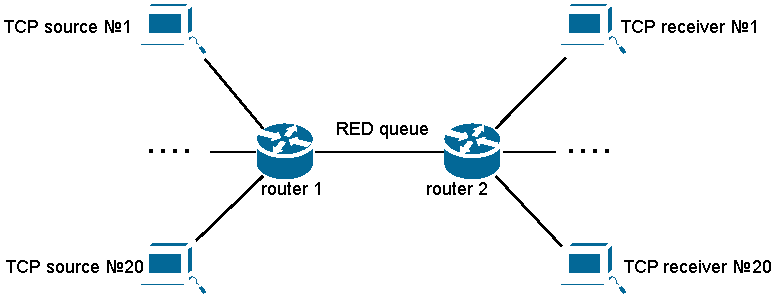
\includegraphics[width=0.7\textwidth]{topology}}
 \caption{Схема топологии моделируемой сети}
\label{ch3:fig1}
\end{figure}

Для данной топологии задали следующие параметры:

\begin{itemize}
\item между TCP-источниками и первым маршрутизатором дуплексные соединения 
	с пропускной способностью 100 Мбит/с и
  	задержкой 20 мс очередью типа DropTail;
\item между TCP-приёмниками и вторым маршрутизатором установлены
  	дуплексные соединения с пропускной способностью 100 Мбит/с и
  	задержкой 20 мс очередью типа DropTail;
\item между маршрутизаторами установлено симплексное соединение
  	($R1$--$R2$) с пропускной способностью 20 Мбит/с и задержкой 15 мс
  	очередью типа RED, размером буфера 300 пакетов; в обратную сторону~---
  	симплексное соединение ($R2$--$R1$) с пропускной способностью 15 Мбит/с и
  	задержкой 20 мс очередью типа DropTail;
\item параметры алгоритма RED: $q_{\min}=75$, $q_{\max}=150$, $q_w=0,002$, $p_{\max}=0.1$;
\item максимальный размер TCP-окна 32; размер передаваемого пакета 1000 байт;
  	байт; время моделирования~---100 единиц модельного времени.
\end{itemize}

\section{Моделирование сети в NS-2}
\label{chap3:sec1}

В имитационной модели TCP-приемники/источники, а также маршрутизаторы реализованы как стандартные узлы, данные передаются по протоколу FTP поверх TCP-Reno, 
для получения данных используются стандартные в программе средства, графики визуализируются в xgraph(для быстрого просмотра) и в GNUPLOT(для дальнейшего анализа).
Модифицированный NS-2 представлен в репозитории ~\cite{ns2-with-red}.

В файле nodes.tcl создаются узлы, задаются их соединения, а также настраиваются агенты и приложения на данные узлы. 
В файле queue.tcl на соеденение между маршрутизаторами накладывается RED, и описываются все его метрики. В файле TCP.tcl 
прописана функция для мониторинга таких метрик TCP, как cwnd, rtt и rtt\_var. В файле nam.tcl представлено создание nam файла для 
визуализации топологии. В файле timing.tcl задаются время моделирования. В файле finish.tcl описана процедура завершения. 
Все данные выводятся в каталог output, а графики в формате pdf c помощью скрипта GNUPLOT выводятся в каталог results. 
Все эти скрипты, запускающиеся с помощью головного файла main.tcl, представлены в Приложении.

Запустив первую модель с заданными параметрами, получили следующие результаты ~\ref{ch3:fig2}.

\begin{figure}[h!]
 \centerline{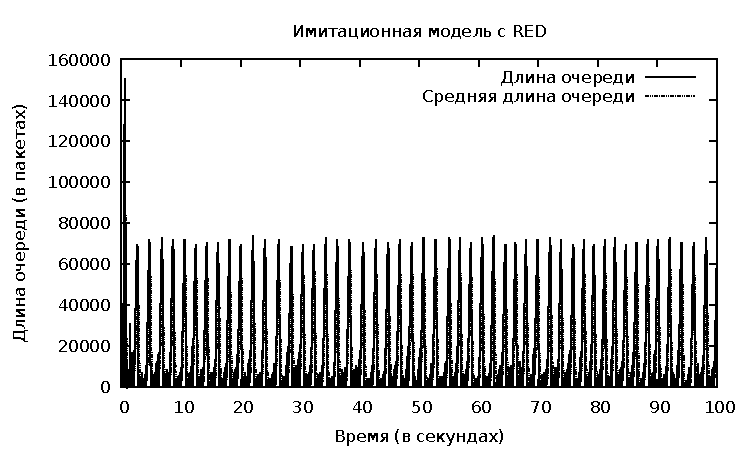
\includegraphics[width=0.7\textwidth]{queues_red}}
 \caption{График длины очереди и средней длины очереди на линке между маршрутизаторами}
\label{ch3:fig2}
\end{figure}


Для проведения сравнительного анализа различных алгоритмов, относящихся к семейству RED, 
было выполнено моделирование аналогичной топологии, время масштабировано до первых 25 секунд для большей наглядности. В результате получили следующие значения размера онка перегрузки, см. рис.
~\ref{ch3:fig3}. В данном примере все алгоритмы, кроме DS-RED, показали крайне
схожие результаты обработки очереди. DS-RED начинает отбрасывать пакеты более
агрессивно из-за своего промежуточного значения $q_{mid}$.

\begin{figure}[h!]
  \centering
  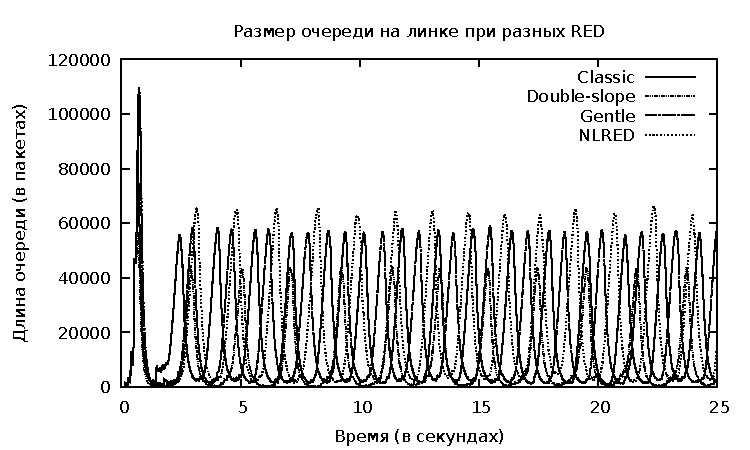
\includegraphics[width=0.7\linewidth]{red1}
  \caption{Длина очереди при разных алгоритмах RED}
  \label{ch3:fig3}
\end{figure}


Кроме того, были изучены результаты, полученные для адаптивных вариантов алгоритмов, детализированные на рисунке~\ref{ch3:fig4}. 
Как мы видим, при автоматической настройке данных средняя длина очереди с течением моделирования не снижается так, как с другими модификациями.
Адаптивные алгоритмы позволяют избежать минусов классического алгоритма RED,
путем:

\begin{itemize}

\item Автоматической установки минимального порога $q_{\min}$. Он
  устанавливается в зависимости от пропускной способности канала и задержки
    целевой очереди.

\item Автоматической установки максимального порога $q_{\max}$. Он
  устанавливается в зависимости от значения $q_{\min}$, причем $q_{\max} = 3*q_{\min}$.

\item Адаптивной настройки $p_{\max}$. Он адаптирован в соответствии с текущей
  средней длиной очереди.

\end{itemize}

\begin{figure}[h!]
  \centering
  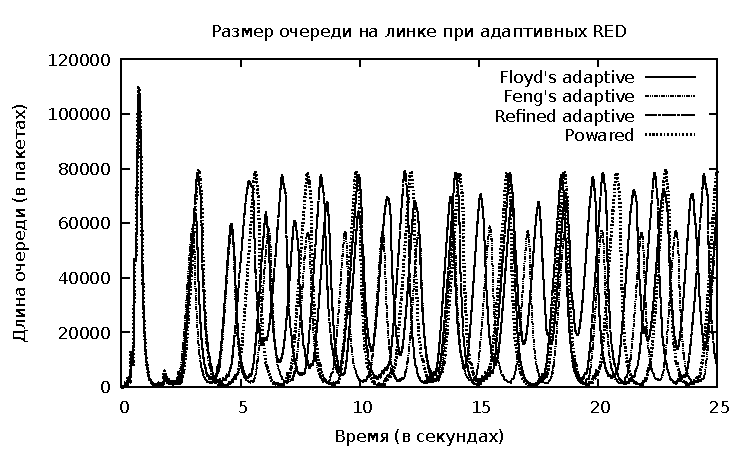
\includegraphics[width=0.7\linewidth]{red2}
  \caption{Адаптивные варианты RED}
  \label{ch3:fig4}
\end{figure}



\section{Моделирование сети в Mininet}
\label{chap3:sec2}

Модель в Mininet более сложная в реализации. В нем используются реальные виртуальные маршрутизаторы 
из класса LinuxRouter, использованы коммутаторы для подсоединения к маршрутизаторам нескольких оконечных 
устройств, а также настроена ip-адресация для корректной работы программы. Для настройки очереди использован 
tc в которой реализованы только модийикации RED и ARED, передача пакетов происходит с помощью iperf3 и 
выводятся в json файл, из которой данные извлекаются с помощью shell скрипта из ~\cite{iperf3-plotter}. 
Также для моделирования программа обращаяется к ядру операционной системы, для того, чтобы изменить тип и размер
окна TCP. Для запуска на нескольких устройствах используются паралельные потоки. Для визуализации также используется GNUPLOT.
Также стоит учитывать, что при реальном моделировании, в отличие от имитационной, результаты могут отличаться при разных запусках,
так как условия не являются идеальными.  

\section{Сравнение результатов в двух средствах моделирования}
\label{chap3:sec3}

Рассмотрим количество отброшенных пакетов в двух средствах. Как показано на Рисунках~\ref{fig:image1} и~\ref{fig:image2}, 
поведение системы в NS-2 и Mininet имеет значительные различия в отношении количества отброшенных пакетов.

\begin{figure}[ht]
    \centering
    % Первый рисунок
    \begin{minipage}[b]{0.45\textwidth}
        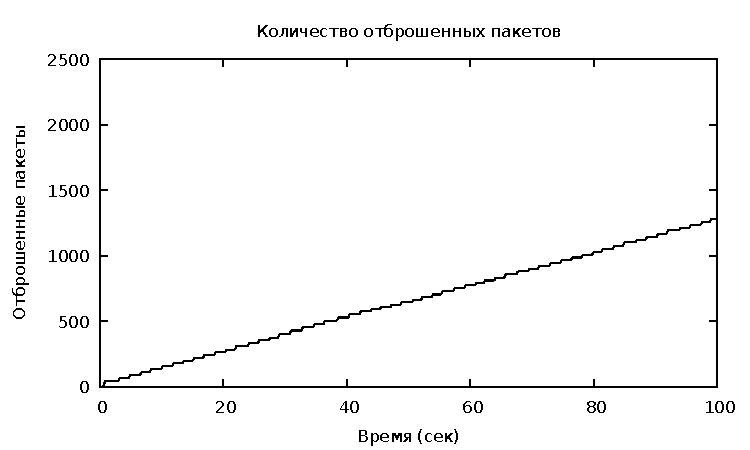
\includegraphics[width=\textwidth]{drops_NS2}
        \caption{Отброшенные пакеты в NS-2}
        \label{fig:image1}
    \end{minipage}
    %\hfill % Добавляет пробел между изображениями, если это необходимо
    % Второй рисунок
    \begin{minipage}[b]{0.45\textwidth}
        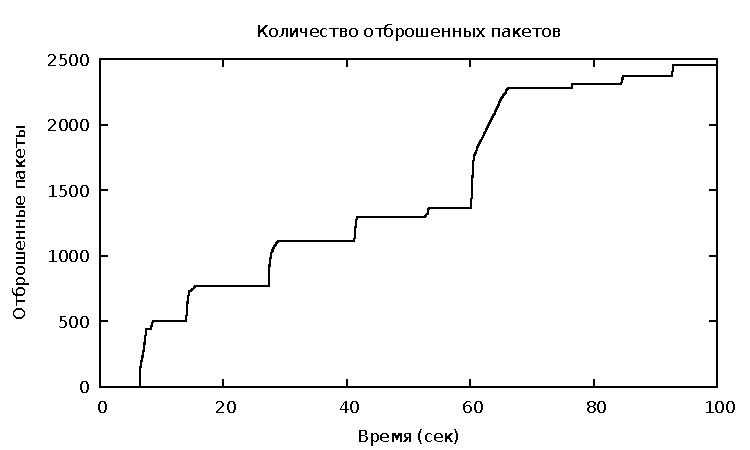
\includegraphics[width=\textwidth]{drops_mininet}
        \caption{Отброшенные пакеты в mininet}
        \label{fig:image2}
    \end{minipage}
\end{figure}

Как мы видим, при натурном моделировании отбрасываются больше пакетов, 
а более плавное изменение графика в NS-2 обьяснется тем, что мониторинг
данных происходит с большей частотой.  



%%% Local Variables:
%%% mode: latex
%%% coding: utf-8-unix
%%% TeX-master: "../default"
%%% End:
